Panel logowania umożliwia uwierzytelnienie z użyciem serwisu GitHub.
Po kliknięciu przycisku ”Zaloguj” użytkownik jest przekierowywany na stronę logowania GitHub.
W~serwisie można zalogować się poprzez podanie adresu e-mail bądź nazwy użytkownika i hasła.
Należy też wyrazić zgodę na przetwarzanie danych przez platformę.
Po poprawnym zalogowaniu użytkownik zostaje przekierowany z powrotem na stronę platformy.
Po przetworzeniu danych uwierzytelniających przez platformę użytkownikowi wyświetlany jest kolejny ekran, zależny od jego uprawnień.
Na rysunku \ref{fig:log_in_button} i \ref{fig:log_in_github} zostały przedstawione kolejne ekrany związane z procesem logowania.

\begin{figure}[H]
    \centering
    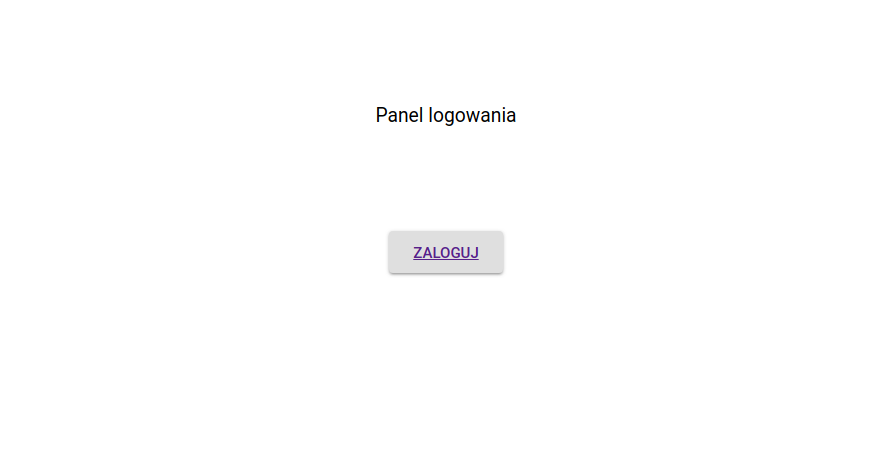
\includegraphics[width = 13cm]{back/log_in_button.png}
    \caption{Ekran logowania w ramach platformy.}
    \label{fig:log_in_button}
\end{figure}

\vfill
\pagebreak

\begin{figure}[H]
    \centering
    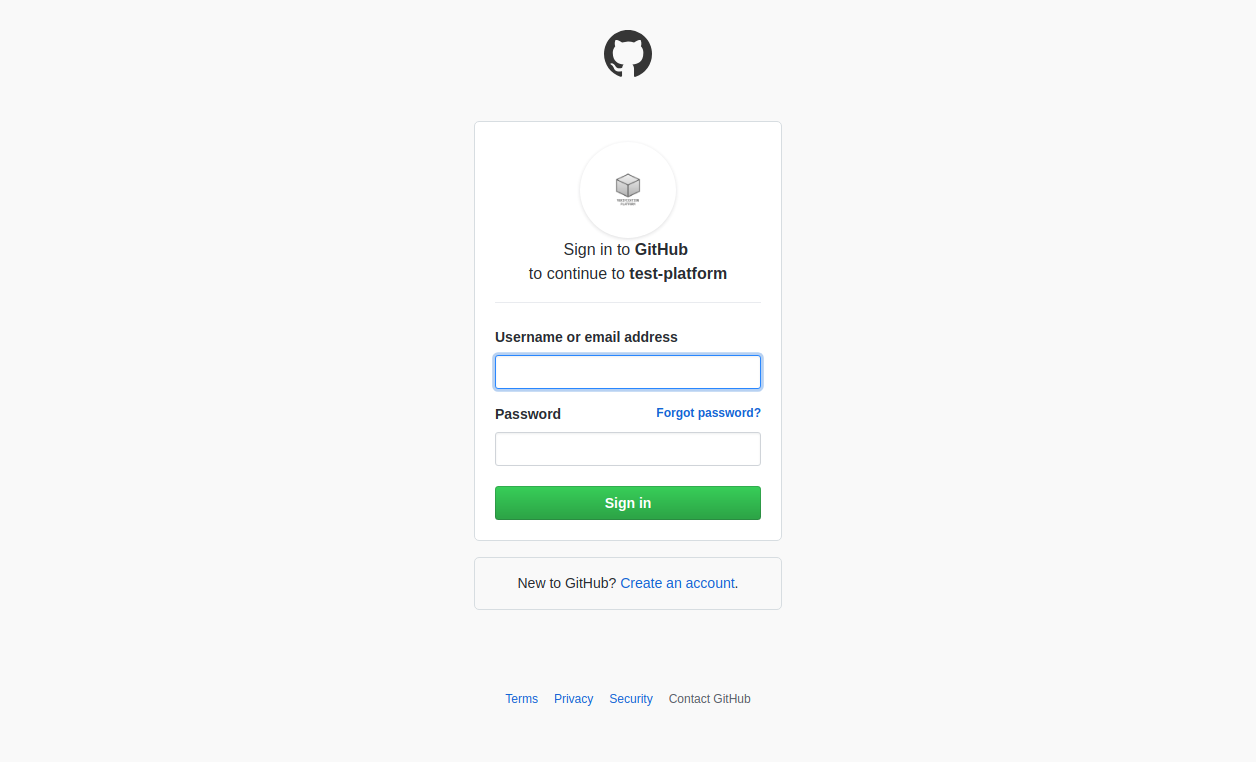
\includegraphics[width = 13cm]{back/log_in_github.png}
    \caption{Ekran logowania do serwisu GitHub.}
    \label{fig:log_in_github}
\end{figure}


